\documentclass[journal, onecolumn, a4paper, 11pt]{IEEEtran}
\usepackage{graphicx} % Required for inserting images
\usepackage[T1]{fontenc}
\usepackage[spanish,es-tabla]{babel}
\decimalpoint
\usepackage{authblk}
\usepackage{enumerate}
\usepackage{lmodern}
%\usepackage{fixcmex}
\usepackage{amsmath}
\usepackage{graphicx}
\usepackage{booktabs}
%\usepackage{diagbox}
\usepackage{caption}
\usepackage{multicol}
\usepackage{multirow}
\usepackage{hyperref}
\usepackage{cite}
\usepackage{listings}
%\usepackage{subfig}
\usepackage{lipsum}
\usepackage{verbatim}
\usepackage{subcaption}
\usepackage[dvipsnames]{xcolor}
\usepackage[backend=biber]{biblatex}

% \addbibresource{Bib.bib}

\title{\textbf{Programación en CUDA} \\\vspace*{10pt} \normalsize  \today{}}

% \title{\textbf{Programación en CUDA}}
    \author[1]{Arias Polanco, Emmanuel}
    \author[1]{Martínez Arévalo, Juan Sebastián}
    \author[1]{Marín Rincón, David Alejandro}
    \author[1]{Prieto Ramírez, Tania Estefania}
\affil[1]{Departamento de Física, Universidad Nacional de Colombia, Bogotá D.C., Colombia}
% \date{\today}

\begin{document}

    \renewcommand{\theequation}{eq. \thesection.\arabic{equation}}
    \renewcommand{\thefigure}{ \thesection.\arabic{figure}}
    \renewcommand{\thetable}{\thesection.\arabic{table}}
    \renewcommand{\thesubsection}{\thesection.\arabic{subsection}}
    \renewcommand{\thesection}{\arabic{section}}

    \definecolor{colorino}{HTML}{1a5220}

\maketitle

\begin{center}
    \textcolor{colorino}{\textbf{Resumen}}
\end{center}

El presente proyecto consiste en la implementación de un algoritmo simple para la realización de operaciones con elementos de matrices aprovechando el poder de la paralelización. El artículo pretende servir como una muestra de los avances realizados al momento de la entrega.

\section{\textbf{Introducción}}

La ejecución de tareas que constan de múltiples procesos que es posible desarrollarlos de manera independiente pueden ser altamente optimizados si dichos procesos son llevados a cabo simultáneamente, dicha forma de cómputo es cobijada bajo el concepto de paralelización. La paralelización de los programas representa uno de los mayores avances en lo que al alto rendimiento de los mismos se refiere, esto ha abierto la posibilidad de obtener resultados que no eran factibles en tiempos razonables para un ser humano. Debido a su importancia y aplicabilidad es fundamental el desarrollo de habilidades en torno su implementación, en particular en la computación científica. El presente proyecto ahonda en dicha labor haciendo uso del software \texttt{CUDA} que permite la paralelización de tareas mediante el uso de GPU's fabricadas por la compañía NVIDIA.

\section{\textbf{Objetivos}}

\subsection{\textbf{Objetivo general}}

Hacer uso del software \texttt{CUDA} para la implementación de programas que permitan aprovechar las ventajas de la paralelización en tarjetas gráficas en problemas de álgebra lineal como la multiplicación y suma de arreglos.

\subsection{\textbf{Objetivos específicos}}

\begin{itemize}
    \item Implementar algoritmos básicos para la manipulación de datos asociados a objetos propios del álgebra lineal.
    \item Analizar el costo temporal del programa para distintos tamaños del mismo y distinto número de núcleos (strong scaling y weak scaling).
    \item Comparar el rendimiento de nuestra implementación paralelizada en GPU, respecto al mostrado por librerías de uso común (\texttt{Eigen}).
    \item Implementar la ejecución para ser realizada por medio del gestionador de recursos \texttt{Slurm}.
\end{itemize}

\section{\textbf{Implementación}}

El programa desarrollado tiene como objetivo la multiplicación de dos matrices, realizando dicha labor de forma paralelizada en una tarjeta gráfica NVIDIA RTX A4500. El algoritmo implementado para la realización de la multiplicación de matrices corresponde a la definición convencional de producto matricial, donde la componente $i,j$ de la matriz resultado es obtenida mediante el producto de la fila $i-ésima$ de la primera matriz por la columna $j-ésima$ de la segunda matriz (siendo dicho producto equivalente al producto punto entre la traspuesta de la fila por la columna), como es mostrado en la figura \ref{fig:enter-label}. En la implementación en paralelo realizada, cada thread de la tarjeta gráfica calcula un componente de la matriz resultado.

\begin{figure}[!h]
    \centering
    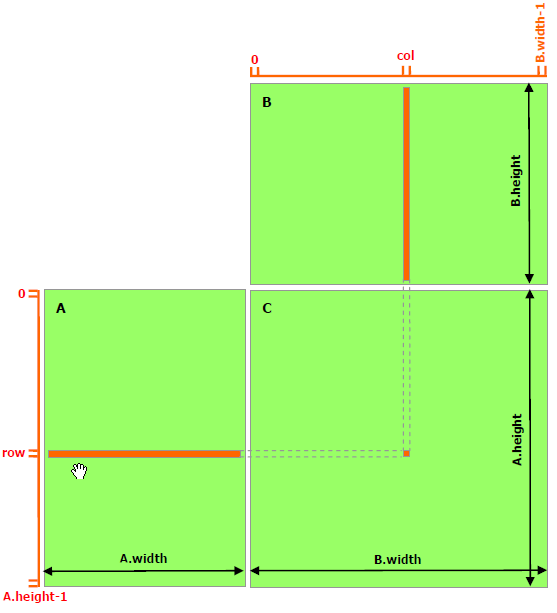
\includegraphics[width=0.5\linewidth]{figs/aux/matrix-multiplication-without-shared-memory.png}
    \caption{Representación gráfica del algoritmo utilizado para la multiplicación de matrices. Imagen tomada de \url{https://docs.nvidia.com/cuda/cuda-c-programming-guide/index.html}.}
    \label{fig:enter-label}
\end{figure}

Bajo esta implementación, se miden los tiempos de cálculo del producto matricial en la GPU, usando el CPU timer de la librería \texttt{chrono} de \texttt{C++}, y el método \texttt{cudaDeviceSynchronize()} del kit de desarollo de \texttt{CUDA}, como se puede apreciar en la figura \ref{strong-matmul}.

\begin{figure}[h!]
    \centering
        \includegraphics[width = 0.55\linewidth]{figs/matmul-strong.pdf}
    \caption{Escalamiento para el problema de multiplicación de matrices cuadradas con distintos tamaños de matriz. Se muestran, en la misma gráfica, las curvas en escala semi logarítmica en el eje $y$ (en color rojo y con marcadores circulares), y sin ella (en color azul y marcadores como estrellas).}
    \label{strong-matmul}
\end{figure}

\newpage

El escalamiento en la figura \ref{strong-matmul} se realiza hasta el tamaño de matriz \texttt{29000x29000} porque este representa la limitación encontrada en el hardware utilizado. Con este tamaño, $\sim19.5GB$ de VRAM de los $\sim20GB$ disponibles en nuestra tarjeta gráfica, se encuentran en uso, como se aprecia en la figura \ref{vram-consumpt}.

\newpage

\begin{figure}[h!]
    \centering
        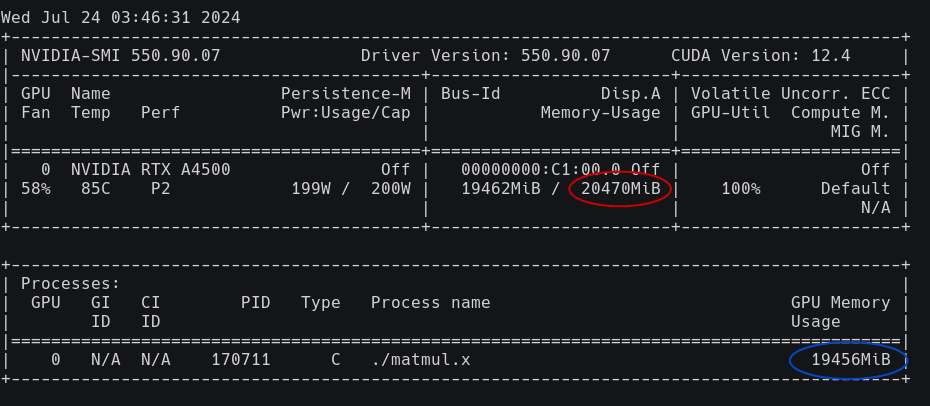
\includegraphics[width=0.8\linewidth]{figs/aux/vram-consumpt.png}
    \caption{Interfaz del Gestor de Sistema de Nvidia (nvidia-smi). Se observa el consumo de VRAM para el cálculo del producto matricial con dos matrices cuadradas de tamaño \texttt{29000x29000} (encerrado en color azul), respecto al total disponible de memoria VRAM (encerrado en color rojo), \texttt{19546/20470 MiB}}
    \label{vram-consumpt}
\end{figure}

Los códigos empleados y necesarios para reproducir estos resultados, se encuentran bajo actualización en el repositorio \url{https://github.com/jmartinezar/Proyecto-final}, listos para generar los datos para el análisis de escalamiento en una máquina con soporte para \texttt{CUDA}. En el archivo comprimido adjunto, bajo el nombre \texttt{proyecto-final-G3.zip}, se encuentran los scripts, los datos y las figuras obtenidas en la ejecución en la máquina empleada para el proyecto.

\begin{figure}[h!]
    \centering
        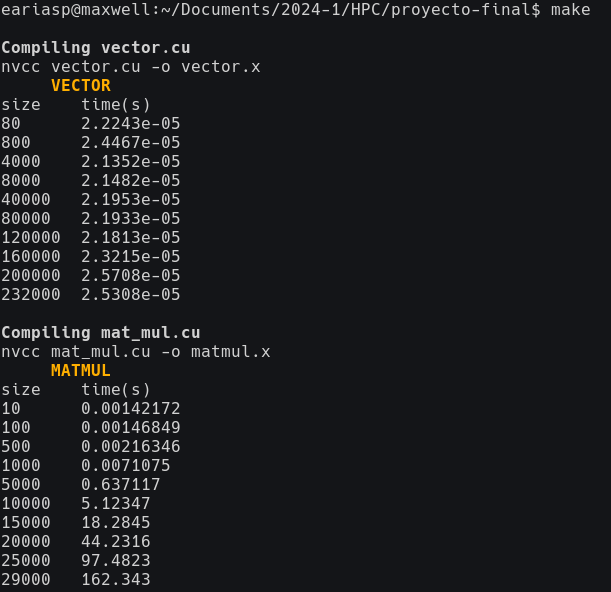
\includegraphics[width=0.6\linewidth]{figs/aux/termout.png}
    \caption{Output obtenido en la terminal al ejecutar el comando \texttt{make}. El comando es ejecutado en el servidor del \textit{Centro de Excelencia en Computación Científica} de la Universidad Nacional de Colombia.}
    \label{termout}
\end{figure}

La reproducción de los datos para ser graficados, se puede lograr con la ayuda del \texttt{Makefile} adjunto, bajo el comando \texttt{make}, como se aprecia en la figura \ref{termout}. La gráfica en la figura \ref{strong-matmul}, generada con \texttt{Python}, puede ser generada haciendo uso del mismo \texttt{Makefile}, mediante el comando \texttt{make plot} en terminal.

\end{document}